\documentclass[
	%a4paper, % Use A4 paper size
	letterpaper, % Use US letter paper size
]{jdf}

\addbibresource{references.bib}

\author{Siddhant Narang}
\email{snarang37@gatech.edu}
\title{RPM Project: Milestone 1}

\begin{document}
%\lsstyle

\maketitle

\section{Introduction}
It surprises me how far we, as humans, have come in the journey of discovering our minds, given the contraints and complexity of the whole thing.
\\“Raven's Progressive Matrices (often referred to simply as Raven's Matrices) or RPM is a non-verbal test typically used to measure general human intelligence and abstract reasoning and is regarded as a non-verbal estimate of fluid intelligence\citep{bilker2012}.”\footnote{\href{https://en.wikipedia.org/wiki/Raven's_Progressive_Matrices}{Definition} taken from Wikipedia}
The test was originally developed by John C. Raven in 1936 \citep{raven1936} and has 60 questions organised in ascending order of difficulty.\\
In this project we will be using a modified version of RPM to test the intelligence of a computer program (agent). Through this project we will externalize human ideas, pack them into an agent and test how 'intelligently' it behaves. \\ This document describes my initial attempt at designing such an agent, based on the techniques and knowledge I have gained until now in CS7637: Knowledge Based Artificial Intelligence. First we will take a look at my attempts at solving a couple of problems and the heuristics I discovered in the process. Then, we will go over the agent's design, and the challenges I faced while designing. After that we will evaluate the design based on two parameters:
\begin{itemize}
	\item Explainability: Is the design able to express in clear terms the path the agent will take while solving the problems ?
	\item Level of Abstraction: Is the design accurately (without going into unnecessary details) able to express the relations and working of different parts ?
\end{itemize}
In the end we will discuss a few future enhancements which can help overcome limitations of the current design.

\section{Human Way of Solving}
While solving these problems I forced myself to think like a child, assuming very little knowledge about the outside world. As I solved the problems, I had to explain each step in detail to the child (myself), giving decriptions and labels of the concepts being used.

\subsection{Solution of a 2x2 Matrix Problem} % This can be purely in figures
\begin{figure}[h]
	\centering
	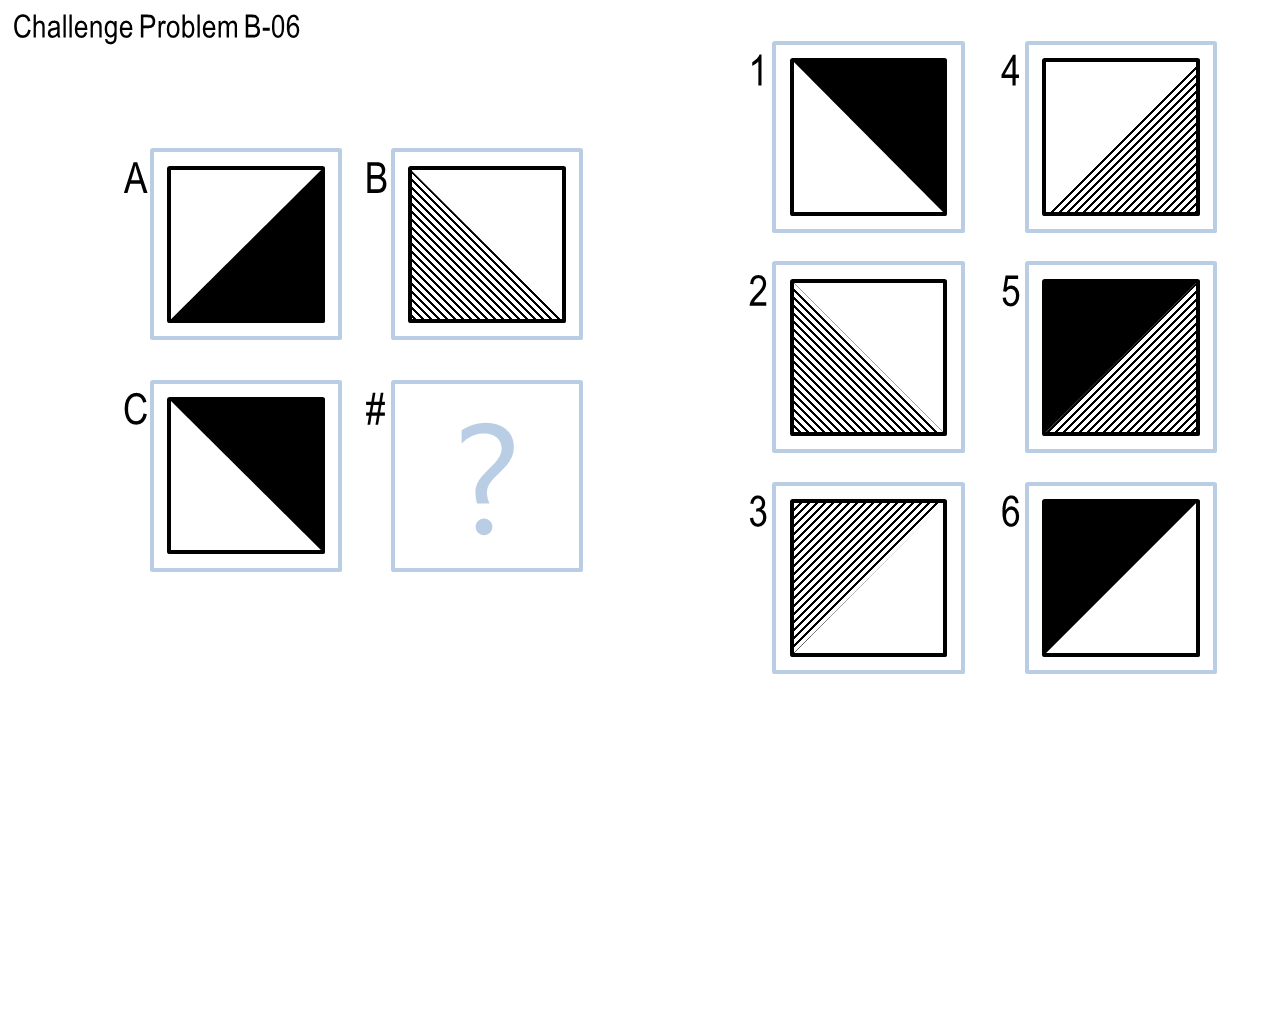
\includegraphics[height=6cm]{Figures/Challenge_Problem_B-06.PNG}
	\caption{A 2x2 matrix problem with horizontal, vertical and digonal relationships}
	\label{fig:problem_2x2}
\end{figure}
Before going into the step wise solution of the problem, I had to describe to the child, in me, what it was seeing in figure \ref{fig:problem_2x2}. Starting with the shape labelled as A:
\begin{itemize}
	\item It is a closed shape with definite boundaries.
	\item It has been divided into two parts by filling one side with black colour.
	\item The side with the black colour is facing the shape with label B.
\end{itemize}
Moving onto the shape with label B:
\begin{itemize}
	\item It looks like shape A.
	\item The colour that divides the shape is not uniform (lines are visible).
	\item The shaded part faces A.
\end{itemize}
Similarly for C, the shape and shade is same as that of A. But the shaded region is facing the side where shape with label \# exists. Now, that we have some descriptions of all the shapes, lets try and decide which shape from labels 1-6 will replace \#-
\begin{enumerate}
	\item The shape which will replace \# should be same as A, B or C
		\begin{itemize}
			\item All shapes from 1-6 are identical to A.
		\end{itemize}
	\item The shape should be divided such that one side is painted and other side is not.
     	\begin{itemize}
     		\item Shapes 1, 2, 3, 4 \& 6 have this feature.
 		\end{itemize}
	\item The shaded region of the shape should face shape C, as A faces B, B faces A, C faces \#, so, \# should face C.
		\begin{itemize}
			\item Shapes 2 and 3 have this feature.
		\end{itemize}
	\item Now, which one should be chosen to replace \# ? We have compared all the features we saw, did we miss something ?
		\begin{itemize}
			\item Yes, if look at shapes 2 and 3, the direction of shading is different. The point where shading begins in 2, is facing away from where 2 is written, and the same point in 3 is facing towards where 3 is written.
			\item Loking at shapes A, B \& C we see the point where shading begins are as close to each other as possible.
		\end{itemize}
	\item Hence, from 2 and 3 the answer should be shape in which the point where shading begins is close to the other shapes, when the figure replaces \#, that is, 3.
\end{enumerate}

\subsection{Solution of a 3x3 Matrix Problem} % This can be purely in figures
\begin{figure}[h]
	\centering
	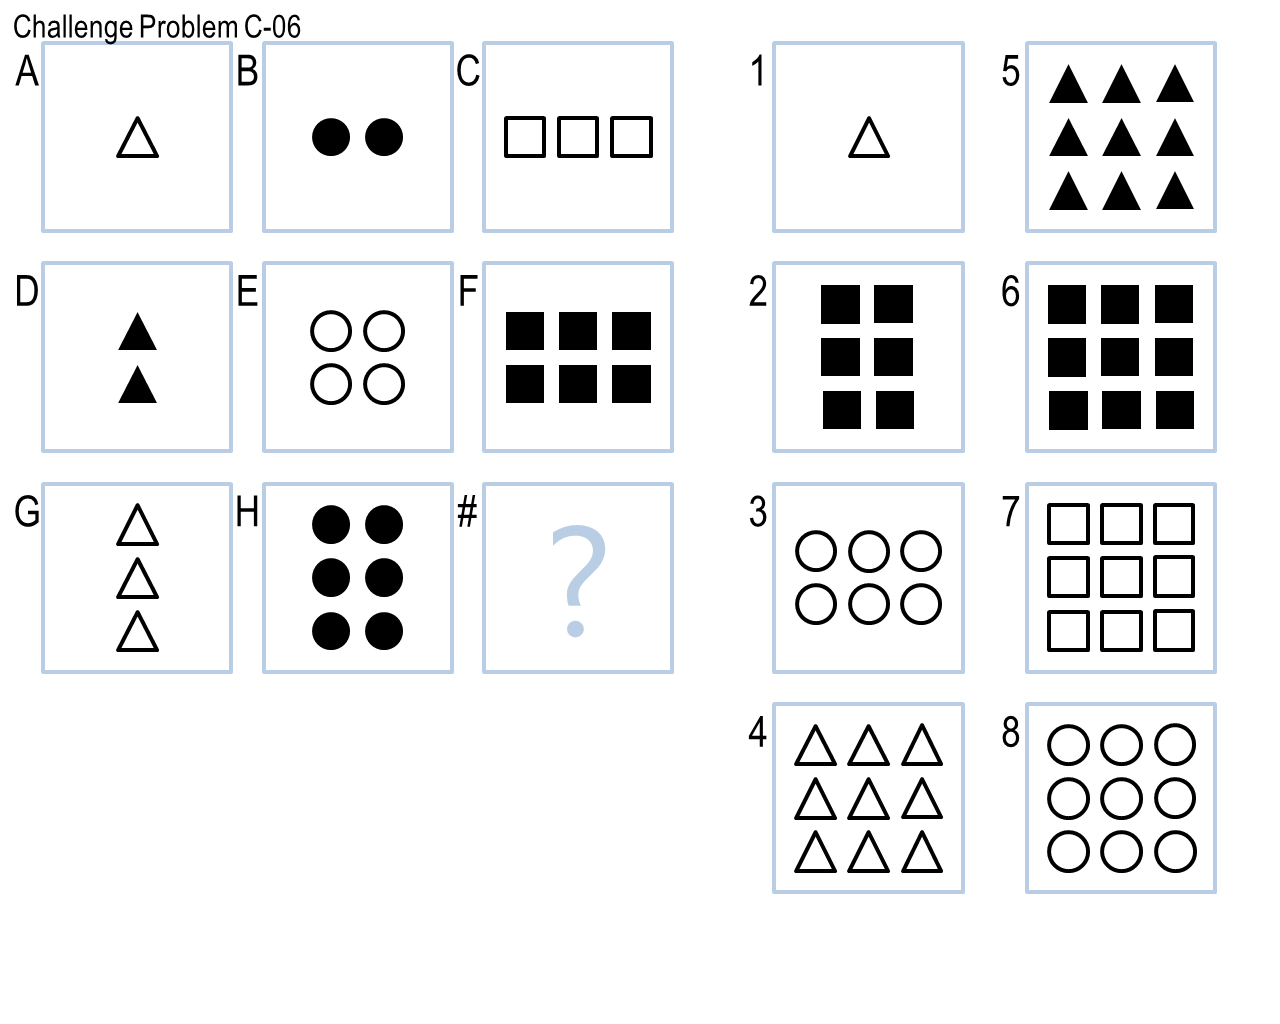
\includegraphics[height=6cm]{Figures/Challenge_Problem_C-06.PNG}
	\caption{A 3x3 matrix problem with horizontal, vertical and digonal relationships}
	\label{fig:problem_3x3}
\end{figure}
\subsection{Useful Heuristics}


\section{Agent Design}
\subsection{Challenges}
\subsection{Knowledge Representation}
\subsubsection{Lexicon}
\subsubsection{Structure}
\subsubsection{Semantics}
\subsection{Problem Solving Technique}
\subsubsection{Generate and Test}
\subsubsubsection{Approach}
\subsubsubsection{Evaluation of Approach}

\section{Design Evalutaion}
\subsection{Explainability}
\subsection{Level of Abstraction}

\section{Future Enhancements}




\begin{table}[h] % [h] forces the table to be output where it is defined in the code (it suppresses floating)
	\caption{Mathematical constants. Notice how the approximations align at the decimal.}
	\small % Reduce font size
	\centering % Centre the table
	\begin{tabular}{L{0.17\linewidth} C{0.12\linewidth} L{0.17\linewidth} L{0.4\linewidth}}
		\textbf{Name} & \textbf{Symbol} & \textbf{Approximation} & \textbf{Description} \\
		\toprule[0.5pt]
		Golden ratio & $\phi$ & 1.618 & Number such that the ratio of " to the number is equal to the ratio of its reciprocal to 1\\
		\midrule
		Euler's number & $e$ & 2.71828 & Exponential growth constant\\
		\midrule
		Archimedes' constant & $\pi$ & 3.14 & The ratio between circumference and diameter of a circle\\
		\midrule
		One hundred & A+ & 100.00 & The grade we hope you’ll all earn in this class\\
	\end{tabular}
\end{table}


\begin{quotation}
	\noindent “Whether or not the grades generated by peers are reliably similar to grades generated by experts is only one factor worth considering, however. Student perception is also an important factor. A recent study indicated that reliance on peer grading is one of the top drivers of high MOOC dropout rates. This problem may be addressed by reintroducing some expert grading where possible.” %\citep{joyner2016}
\end{quotation}


\begin{itemize}
	\item First bullet point item
	\item Second bullet point item
\end{itemize}

Numbered list:

\begin{enumerate}
	\item First numbered item
	\item Second numbered item
\end{enumerate}

\section{Procedural elements}
\subsection{In-line citations}
Articles or sources to which you refer should be cited in-line with the authors’ names and the year of publication.\footnote{In-line citations are preferred over footnotes, and we favor APA citation format for both in-line citations and reference lists. Refer to the Purdue Online Writing Lab, or follow the above examples. Footnotes should use 8.5 point text with 14 point line spacing.} The citation should be placed close in the text to the actual claim, not merely at the end of the paragraph. For example: students in the OMSCS program are older and more likely to be employed than students in the on-campus program \citep{joyner2017}. In the event of multiple authors, list them. For example: research finds sentiment analysis of the text of OMSCS reviews corresponds to student-assigned ratings of the course \citep{newman2018}. You may also cite multiple studies together. For example: several studies have found students in the online version of an undergraduate CS1 class performed equally with students in a traditional version (\cite{joyner2018a}; \cite{joyner2018b}). If you would like to refer to an author in text, you may also do so by including the year (in parentheses) after the author’s name in the text. If a publication has more than 4 authors, you may list the first author followed by ‘et al.’ For example: \citeauthor{joyner2016} (\citeyear{joyner2016}) claim that a round of peer review prior to grading may improve graders’ efficiency and the quality of feedback given. This applies to parenthetical citations as well, e.g. \citep{joyner2016}.

\section{References}
\printbibliography[heading=none]

\section{Appendices}
You may optionally move certain information to appendices at the end of your paper, after the reference list. If you have multiple appendices, you should create a section with a \emph{Heading 1} of “Appendices.” Each appendix should begin with a descriptive \emph{Heading 2}; appendices can thus be referenced in the body text using their heading number and description, e.g. “Appendix 5.1: Survey responses.” If you have only one appendix, you can label it with the word “Appendix” followed by a descriptive title, e.g., “Appendix: Survey responses.”

These appendices do not count against the page limit, but they should not contain any information required to answer the question in full. The body text should be sufficient to answer the question, and the appendices should be included only for you to reference or to give additional context. If you decide to move content to an appendix, be sure to summarize the content and note it in relevant place in the body text, e.g., “The raw data can be viewed in \emph{Appendix 5.1: Survey responses}.”

\end{document}